In this section, we introduce the relevant control background needed for the remainder of the paper, and we detail how the controller and the system behave under normal operation.

\begin{figure}[t]
\centering
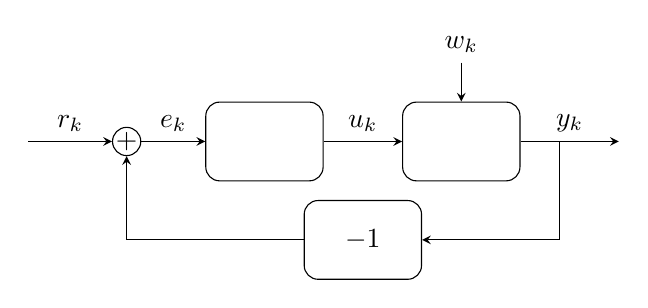
\begin{tikzpicture}[>=stealth]
\coordinate (start) at (-1.25,0);
\coordinate (end) at (6.25,0);
\coordinate (feedbackstart) at (5.5,0);
\coordinate (noisestart) at (4.25,1);

\node[circle, draw, inner sep=0, minimum size=0.3cm] (sum) at (0,0) {$+$};
%\node[circle, draw, inner sep=0, minimum size=0.3cm] (sumw) at (3.5,0) {$+$};
\node[rectangle, rounded corners=5pt, draw, minimum width=1.49cm, minimum height=1cm] (c) at (1.75,0) {$\ctrler$};
\node[rectangle, rounded corners=5pt, draw, minimum width=1.49cm, minimum height=1cm] (p) at (4.25,0) {$\plant$};
\node[rectangle, rounded corners=5pt, draw, minimum width=1.49cm, minimum height=1cm]
  (neg) at (3.0,-1.25) {$-1$};

\draw[->] (start) -- node[above] {$r_k$} (sum);
\draw[->] (sum) -- node[above] {$e_k$} (c);
\draw[->] (c) -- node[above] {$u_k$} (p);
%\draw[->] (sumw) -- node[above] {} (p);
\draw[->] (p) -- node[above] {$y_k$} (end);
\draw[->] (feedbackstart) |- (neg);
\draw[->] (neg) -| (sum);
\draw[->] (noisestart) node[above] {$w_k$} -- (p);
\end{tikzpicture}

\caption{Control loop: The reference value $r_k$ is compared with the output $y_k$ of the plant $\plant$.
    The control error $e_k = r_k - y_k$ is used by the controller $\ctrler$ to compute the value of the control signal $u_k$.
    The plant is disturbed by the stochastic process $w_k$.}
\label{fig:loop}
\end{figure}

\subsection{Plant Model}

We first describe the model we use for the object we are trying to control.
In control terms---mostly due to historical reasons---this object is called a \emph{plant}.
Examples range from a pendulum that we would like to stabilise in the upward position, to a chemical dilution process, to the distribution of workload in a datacenter.

Plants are usually modelled as continuous- or discrete-time dynamical systems. 
All real-world plants are nonlinear, but for control design purposes they are often linearised around their operating points.
Around such a point, the resulting model becomes a Linear Time-Invariant (LTI) system.
In this paper, we restrict our analysis to discrete-time LTI systems, because we investigate controllers implemented with fixed-rate sampling and actuation in digital electronics.
To design and analyse these systems, we use the discrete-time counterpart of the continuous-time physical model, which can be obtained with standard techniques~\cite{Astrom:1997}.

We consider a plant $\plant$ described in state-space form:
\begin{equation}
\label{eq:background:plant}
    \plant : \left\{
    \begin{aligned}
        x_{k+1} &\,=\,  \Ap\,x_k + \Bp\,u_k + \Wp\,w_k \\
        y_k &\,=\, \Cp\,x_k + \Dp\,u_k
    \end{aligned}
    \right.
\end{equation}

In~\eqref{eq:background:plant}, $k$ counts the discrete instants that represent the plant's sampling points.
We assume periodic sampling; the time between two consecutive samples $k$ and $k+1$ is fixed and equal to sampling period $\Ts$.
In the equation, $x_k$ is a column vector with $n_x$ elements.
These elements represent the state variables that account for, e.g., the storage of mass, momentum, and energy.
Similarly, $u_k$ is a column vector with $n_u$ elements.
These values represent the inputs that affect the dynamics of the plant.
We also consider $w_k$, a column vector with $n_u$ elements.
The term $w_k$ represents an unknown load disturbance, modelled as a stationary stochastic process with known properties.
Finally, $y_k$ is a column vector with $n_y$ elements, that represents the measurements that are taken from our plant.
The matrices $\Ap$ (size $n_x \times n_x$), $\Bp$ (size $n_x \times n_u$), $\Cp$ (size $n_y \times n_x$), $\Dp$ (size $n_y \times n_u$), and $\Wp$ (size $n_x \times n_u$) characterise the dynamics of the plant.

\subsection{Controller Model}

The plant $\plant$ is controlled by a periodically executing controller $\ctrler$ with implicit deadlines, i.e., the deadline of each task instance (job) coincides with the next task activation.
We consider the class of all linear controllers with a one-step delay between sampling and actuation.\footnote{One-step delay controllers are controllers in which a control signal is computed in the $k$-th interval and actuated at the beginning of the $k+1$-th period. In the real-time systems jargon, one-step delay controllers are often referred to as controllers that follow the Logical Execution Time (LET) paradigm~\cite{Kirsch:2012, Ernst:2018}. From the real-time perspective, implementing the controller following the LET paradigm improves the timing predictability. From the control perspective, one-step delay controllers reduce activation jitter and allows the engineer to neglect time-varying computational delays.}
In other words, we consider all the controllers that can be written as linear systems, according to the following state-space equation:
\begin{equation}
\label{eq:background:controller}
    \ctrler : \left\{
    \begin{aligned}
        z_{k+1} &\,=\, \Ac\,z_k + \Bc\,e_k \\
        u_{k+1} &\,=\, \Cc\,z_k + \Dc\,e_k
    \end{aligned}
    \right.
\end{equation}

Here, $z_k$ is a column vector with $n_z$ elements that represents the state of the controller.
The input of the controller is $e_k$, a vector of $n_y$ elements.
Each element in the vector is the error between the corresponding plant output and its reference value ($e_k = r_k - y_k$, where $r_k$ represents the reference values for the plant outputs).
Finally, $u_k$ is a vector of $n_u$ elements, that encodes the output of the controller, which is connected to the plant input vector.
The matrices $\Ac$ (size $n_z \times n_z$), $\Bc$ (size $n_z \times n_y$), $\Cc$ (size $n_u \times n_z$), and $\Dc$ (size $n_u \times n_y$) characterise the dynamics of the controller.
For every task activation, the controller first applies the value of $u_k$ that was computed by the previous job and then reads the inputs $r_k$ and $y_k$.
It then calculates the values of $z_{k+1}$ and $u_{k+1}$ that will be used in the next iteration.

The analysis methodology presented in the remainder of this paper is valid for \emph{all} linear controllers.
The class of linear controllers includes some of the most frequently used controllers in industry, in particular proportional and integral (PI), proportional, integral, and derivative (PID), lead--lag compensators, and linear-quadratic-Gaussian (LQG) controllers.
Although the performance analysis is presented for the time-invariant case, the formulas are valid also for systems with time-varying matrices.
Hence, it is possible to analyse plants and controllers that transition between different local linear models.

\subsection{Closed-Loop System Dynamics}
\label{sec:cldynamics}

We now analyse the closed-loop system shown in Figure~\ref{fig:loop}.
Combining the dynamical models from~\eqref{eq:background:plant} and~\eqref{eq:background:controller}, we obtain matrices that represent the closed-loop system.
We denote the state vector of the closed-loop system with $\tilde{x}_k = \left[ x_k^\T,\, z_k^\T,\, u_k^\T \right]^\T$, where $^\T$ is the transpose operator.
In this way, we obtain a system that has the vectors $r_k$ and $w_k$ as input, and is described by
%
\begin{equation} 
\label{eq:feedback-basic}
    \clsys : \left\{
    \begin{aligned}
        \tilde{x}_{k+1} &\,=\, \tilde A\,\tilde{x}_{k} + B_r\,r_{k} + B_w\,w_{k}\\
        y_{k} &\,=\, \tilde C\,\tilde{x}_{k},
    \end{aligned} \right.
\end{equation}
%
where the closed-loop state matrix $\tilde A$ is \fix{Consider changing $\tilde A$ to something else?}
%
\begin{equation}
\label{eq:matrixA}
    \tilde A =
    \begin{bmatrix} \Ap       & 0_{n_x \times n_z} & \Bp \\
                    -\Bc\,\Cp & \Ac                                      & -\Bc\,\Dp \\
                    -\Dc\,\Cp & \Cc                                      & -\Dc\,\Dp
    \end{bmatrix},
\end{equation}
%
the input matrices $B_r$ and $B_w$ are
%
\begin{equation}
    B_r = \begin{bmatrix} 0_{n_x \times n_y} \\ \Bc \\ \Dc \end{bmatrix},\;\;
    B_w = \begin{bmatrix} \Wp \\ 0_{n_z \times n_u} \\ 0_{n_u \times n_u} \end{bmatrix},
\end{equation}
%
and the output matrix $\tilde C$ is
%
\begin{equation}
    \tilde C = \begin{bmatrix} \Cp & 0_{n_x \times n_z} & \Dp \end{bmatrix}.
\end{equation}
%
Figure~\ref{fig:closedloop} shows the graphical representation of the closed-loop system $\clsys$, with input and output signals.

\begin{figure}[t]
\centering
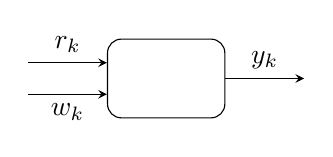
\begin{tikzpicture}[>=stealth]
\node[rectangle, rounded corners=5pt, draw, minimum width=1.49cm, minimum height=1cm] (l) at (0,0) {$\clsys$};

\draw[->] ([xshift=-1cm,yshift=0.2cm]l.west) -- node[above] {$r_k$} ([yshift=0.2cm]l.west);
\draw[->] ([xshift=-1cm,yshift=-0.2cm]l.west) -- node[below] {$w_k$} ([yshift=-0.2cm]l.west);
\draw[->] (l.east) -- node[above] {$y_k$} ([xshift=1cm]l.east);
\end{tikzpicture}

\caption{Closed-loop system rewritten as a new linear system $\clsys$.
    The resulting system has two inputs, $r_k$ and $w_k$ and one output.
    The feedback loop shown in Figure~\ref{fig:loop} is hidden inside $\clsys$.}
\label{fig:closedloop}
\end{figure}

\paragraph*{Stability}

To assess the stability of the closed-loop system under normal operation, it is sufficient to check the eigenvalues of the state matrix. 
According to the Schur stability criterion~\cite{Astrom:1997}, if the eigenvalues of $\tilde A$ lie within the unit disc, then the system is asymptotically stable. 
Formally, a closed-loop system is Schur stable if and only if
\fix{Change definition of \code{\\eig} to not include $\lambda$}
%
\begin{equation}
    \label{eq:schur}
    \max_i{\abs{\eig{i}{\tilde A}}} < 1,
\end{equation}
%
where $\eig{i}{\tilde A}$ is a function that returns the $i$-th eigenvalue of~$\tilde A$.

If the system dynamics change at runtime (e.g., in the case of a lost sample, unexpected delay, or computational problem), Schur stability is no longer a sufficient stability criterion.
Instead, \emph{switching stability analysis} can be employed to check the stability of a system with alternating dynamics~\cite{Jungers2009}.
There has been a lot of research on the switching stability analysis, with multiple tools developed in order to simplify the analysis.
Two main methods are employed: (i) the search for a common Lyapunov function, e.g., as done in~\cite{Linsenmayer:2017}, (ii) the computation of the Joint Spectral Radius (JSR), e.g., as done in~\cite{Maggio:2020,Jungers:2014}.

\paragraph*{Performance}

Alongside stability, it is important to look at the \emph{performance} of the closed-loop system.
Performance can be defined in different ways, often depending on the application~\cite{Astrom:2006}.
Whichever way is chosen, a common way to quantify performance is to define a cost function and evaluate the cost function during the execution of the controller.
In our work, we use a quadratic cost function
%
\begin{equation}
    \label{eq:cost}
    J_k = \E{e_k^\T Q_e e_k + u_k^\T Q_u u_k}.
\end{equation}
%
The cost function penalises deviations from the reference value as well as usage of the control signal.
$\mathbb{E}$ denotes expected value, and the positive semidefinite weighting matrices $Q_e$ (size $n_y \times n_y$) and $Q_u$ (size $n_u \times n_u$) weigh the different terms against each other.
A small cost value means that the controller successfully makes the error approach zero, using a small control signal.

If the stochastic properties of the external signals $r_k$ and $w_k$ are known, it is possible to calculate the value of the cost function analytically.
For simplicity and without loss of generality, we will henceforth assume that $r_k = 0$ (i.e., we want to regulate the output to zero) and that $w_k$ is a zero-mean Gaussian white noise process with variance~$R=\E{w_k w_k^\T}$.
More elaborate disturbance models can be realised by adding extra states in the plant model.

We now detail how to evaluate \eqref{eq:cost}.
Let $P_k$ denote the covariance of the closed-loop state vector at time $k$,
%
\begin{equation}
\label{eq:covarcalc}
    P_k = \E{\tilde x_k \tilde x_k^\T }.
\end{equation}
%
The state covariance evolves according to
%
\begin{equation}
\label{eq:covevolution}
    P_{k+1} = \tilde A \,P_k\, \tilde A^\T + B_w \,R\, B_w^\T.
\end{equation}
%
Given $P_k$, we can calculate the cost for time step $k$ as
%
\begin{equation}
\label{eq:covartocost}
    J_k = \E{\tilde x_k^\T \,Q\, \tilde x_k } = \trace{P_k \,Q},
\end{equation}
%
where $\mathrm{tr}$ computes the trace of the matrix, and
%
\begin{equation}
    \setlength\arraycolsep{2pt}
    Q = \begin{bmatrix} 
        \Cp^\T\,Q_e\,\Cp                           & 0_{n_x \times n_z} & 0_{n_x \times n_u} \\
        0_{n_z \times n_x}  & 0_{n_z \times n_z}   & 0_{n_z \times n_u} \\
        0_{n_u \times n_x} & 0_{n_u \times n_z}  & Q_u
    \end{bmatrix} 
\end{equation}
%
is the total cost matrix.
The stationary cost of the system is defined as $J_\infty$.
This is the cost that the system converges to when operating under normal conditions:
%
\begin{equation}
    J_\infty = \lim_{k\rightarrow\infty} J_k.
\end{equation}
%
This means that there exists an instant $\bar{k}$ for which $J_k$ reaches a value arbitrarily close to the steady-state value $J_\infty$, or $\forall \varepsilon, \,\, \exists \bar{k} \text{~s.t.~} \forall k>\bar{k},\,\,|(J_k - J_\infty)/J_\infty| < \varepsilon$.
